%\documentclass[dvipdfmx]{beamer}      % platex の場合
\documentclass{beamer}                 % lualatex の場合
\usepackage{mySld}
\usepackage{multicol}

\begin{document}
\title{基礎コンピュータ工学\\第5章 機械語プログラミング\\(パート8)}
\date{}

\begin{frame}
  \titlepage
  \centerline{\url{https://github.com/tctsigemura/TecTextBook}}
  \vfill
  \centerline{本スライドの入手:
    \raisebox{-7mm}{
\includegraphics[scale=0.3]{../Img/QRs5_8.png}}}
\end{frame}

%==============================================================================
%\begin{frame}
%  \frametitle
%  \tableofcontents
%\end{frame}

\section{条件ジャンプ命令}
%==============================================================================
\begin{frame}
  \frametitle{ジャンプ命令(7種類)の残り3種類}
  \begin{description}
  \item[無条件ジャンプ命令:]\emph{プログラムの流れ}を指定のアドレスに飛ばす.
    \begin{itemize}
      \item \emph{JMP(Jump)命令}:いつもジャンプする.
    \end{itemize}
    \vfill
  \item[条件ジャンプ命令:]ある条件のときだけジャンプする.
    \begin{itemize}
      \item \emph{JZ(Jump on Zero)命令}:$Z=1$ ならジャンプ
        \vfill
      \item \emph{JC(Jump on Carry)命令}:$C=1$ ならジャンプ
        \vfill
      \item \emph{JM(Jump on Minus)命令}:$S=1$ ならジャンプ
        \vfill
      \item \emph{JNZ(Jump on Not Zero)命令}:$Z=0$ ならジャンプ
        \vfill
      \item \emph{JNC(Jump on Not Carry)命令}:$C=0$ ならジャンプ
        \vfill
      \item \emph{JNM(Jump on Not Minus)命令}:$S=0$ ならジャンプ
    \end{itemize}
  \end{description}
  \vfill
\end{frame}

%==============================================================================
\begin{frame}
  \frametitle{JNZ(Jump on Not Zero)命令}
  Zフラグが0なら(計算結果が0でないなら)ジャンプする.
  \vfill
  \begin{description}
  \item[フラグ:] 変化しない.
    \vfill

  \item[ニーモニック:]\texttt{JNZ EA}~~~~~~~~~\texttt{(if(Z=0) PC ← EA)}
    \vfill

  \item[命令フォーマット:] 2バイトの長さを持つ.\\
    \twoByte{$1011_2$}{$01_2$~\XR}{\A}
    \vfill

  \item[フローチャート:] ある程度,自由にアレンジしてよい.\\
    \centerline{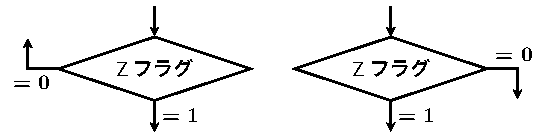
\includegraphics[scale=0.7]{../Tikz/jnz.pdf}}
  \end{description}
  \vfill
\end{frame}

%==============================================================================
\begin{frame}
  \frametitle{JNZ命令の使用例}
  ループを3回,繰り返すプログラム\\
  \vfill
  \begin{minipage}{0.4\columnwidth}
    \centerline{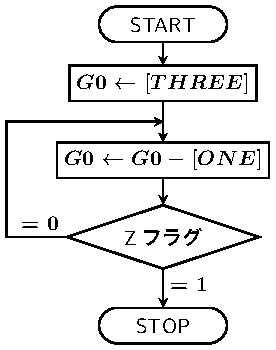
\includegraphics[scale=0.7]{../Tikz/flow0C.pdf}}
  \end{minipage}
  \begin{minipage}{0.59\columnwidth}
    {\ttfamily\small\begin{center}
      \begin{tabular}{|l|l|l|l l|} \hline
        番地 & 機械語 & ラベル & \multicolumn{2}{|c|}{ニーモニック} \\
        \hline
        00 & 10 07 &           & LD   & G0,THREE              \\
        02 & 40 08 &  LOOP     & SUB  & G0,ONE                \\
        04 & B4 02 &           & JNZ  & LOOP                  \\
        06 & FF    &           & HALT &                       \\
        07 & 03    &  THREE    & DC   & 3                     \\
        08 & 01    &  ONE      & DC   & 1                     \\
        \hline
      \end{tabular}
    \end{center}}
  \end{minipage}
  \vfill
  \begin{itemize}
  \item JNZを使用した方が簡単になった.
  \end{itemize}
  \vfill
\end{frame}

%==============================================================================
\begin{frame}
  \frametitle{JZ命令の使用例(比較のために再掲)}
  ループを3回,繰り返すプログラム\\
  \vfill
  \begin{minipage}{0.4\columnwidth}
    \centerline{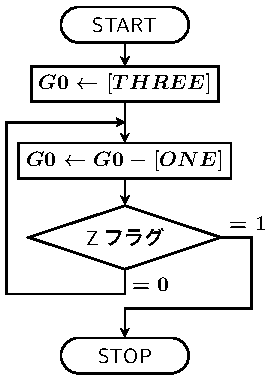
\includegraphics[scale=0.7]{../Tikz/flow0B.pdf}}
  \end{minipage}
  \begin{minipage}{0.59\columnwidth}
    {\ttfamily\small\begin{center}
      \begin{tabular}{|l|l|l|l l|} \hline
        番地 & 機械語 & ラベル & \multicolumn{2}{|c|}{ニーモニック} \\
        \hline
        00 & 10 09 &           & LD   & G0,THREE              \\
        02 & 40 0A &  LOOP     & SUB  & G0,ONE                \\
        04 & A4 08 &           & JZ   & STOP                  \\
        06 & A0 02 &           & JMP  & LOOP                  \\
        08 & FF    &  STOP     & HALT &                       \\
        09 & 03    &  THREE    & DC   & 3                     \\
        0A & 01    &  ONE      & DC   & 1                     \\
        \hline
      \end{tabular}
    \end{center}}
  \end{minipage}
  \vfill
\end{frame}

%==============================================================================
\begin{frame}
  \frametitle{JNC(Jump on Not Carry)命令}
  Cフラグが0なら(オーバーフローしていないなら)ジャンプする.
  \vfill
  \begin{description}
  \item[フラグ:] 変化しない.
    \vfill

  \item[ニーモニック:]\texttt{JNC EA}~~~~~~~~~\texttt{(if(C=0) PC ← EA)}
    \vfill

  \item[命令フォーマット:] 2バイトの長さを持つ.\\
    \twoByte{$1011_2$}{$10_2$~\XR}{\A}
    \vfill

  \item[フローチャート:] ある程度,自由にアレンジしてよい.\\
    \centerline{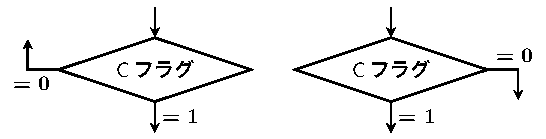
\includegraphics[scale=0.7]{../Tikz/jnc.pdf}}
  \end{description}
  \vfill
\end{frame}

%==============================================================================
\begin{frame}
  \frametitle{JNM(Jump on Not Minus)命令}
  Sフラグが0なら(正かゼロなら)ジャンプする.
  \vfill
  \begin{description}
  \item[フラグ:] 変化しない.
    \vfill

  \item[ニーモニック:]\texttt{JNM EA}~~~~~~~~~\texttt{(if(S=0) PC ← EA)}
    \vfill

  \item[命令フォーマット:] 2バイトの長さを持つ.\\
    \twoByte{$1011_2$}{$11_2$~\XR}{\A}
    \vfill

  \item[フローチャート:] ある程度,自由にアレンジしてよい.\\
    \centerline{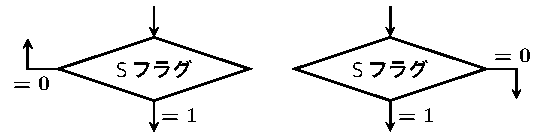
\includegraphics[scale=0.7]{../Tikz/jnm.pdf}}
  \end{description}
  \vfill
\end{frame}

%==============================================================================
%\begin{frame}
%  \frametitle{条件判断1(JNZ使用)}
%  計算結果により処理をするかしないか変化する例
%  \vfill
%  \begin{minipage}{0.49\columnwidth}
%    \begin{itembox}[l]{\footnotesize 計算結果がゼロなら「処理」\emph{しない}}
%      \centerline{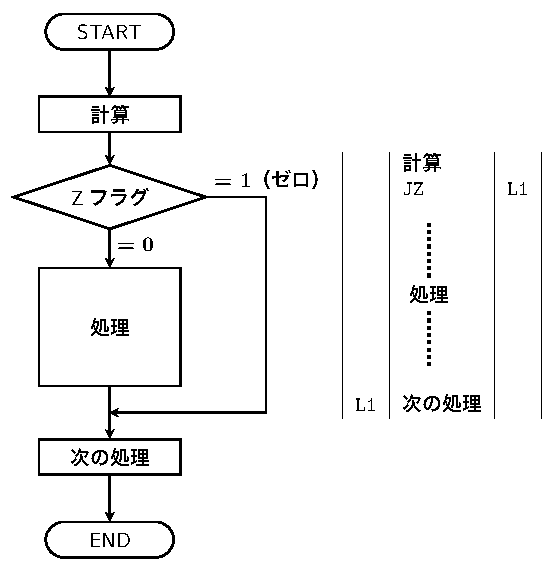
\includegraphics[scale=0.6]{../Tikz/flow2AB.pdf}}
%    \end{itembox}
%  \end{minipage}
%  \begin{minipage}{0.5\columnwidth}
%    \begin{itembox}[l]{\footnotesize 計算結果がゼロなら「処理」\emph{する}}
%      \centerline{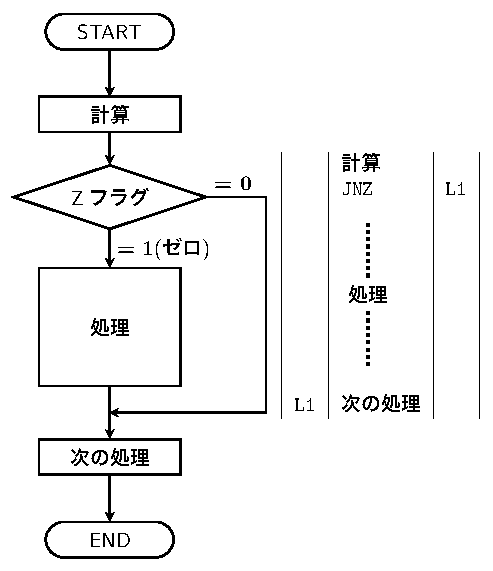
\includegraphics[scale=0.6]{../Tikz/flow2AC.pdf}}
%    \end{itembox}
%  \end{minipage}
%  \vfill
%\end{frame}

%==============================================================================
\begin{frame}
  \frametitle{条件判断の例(JNM使用)}
  絶対値を求めるプログラム(例題5-1の改良)\\
  \vfill
  \begin{minipage}{0.49\columnwidth}
    \centerline{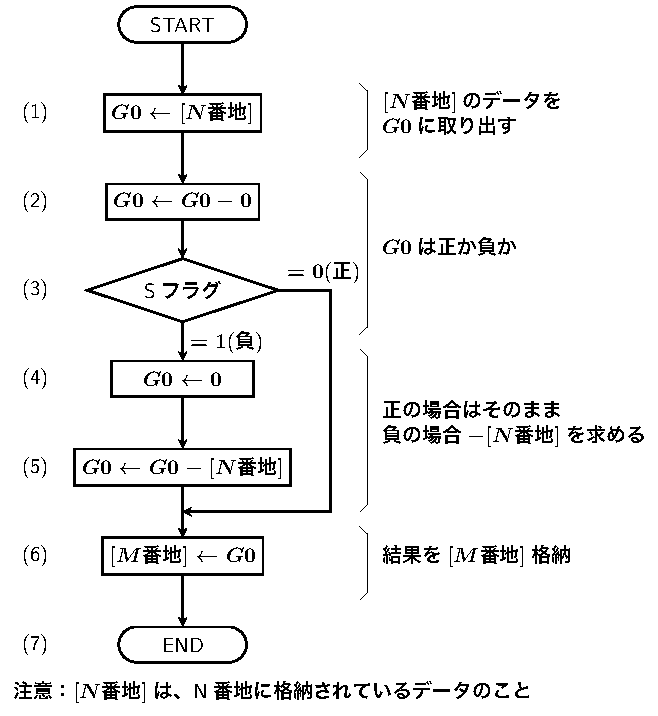
\includegraphics[scale=0.5]{../Tikz/flow1.pdf}}
  \end{minipage}
  \begin{minipage}{0.5\columnwidth}
    {\ttfamily\scriptsize\begin{center}
      \begin{tabular}{|l|l|l|l l|}
        \hline
        番地 & 機械語 & ラベル & \multicolumn{2}{|c|}{ニーモニック} \\
        \hline
        00 & 10 0E & START& LD   & G0,N    \\
        02 & 40 0D &      & SUB  & G0,ZERO \\
        04 & BC 0A &      & JNM  & L1      \\
        06 & 10 0D &      & LD   & G0,ZERO \\
        08 & 40 0E &      & SUB  & G0,N    \\
        0A & 20 0F & L1   & ST   & G0,M    \\
        0C & FF    &      & HALT &         \\
        0D & 00    & ZERO & DC   & 0       \\
        0E & FF    & N    & DC   & -1      \\
        0F & 00    & M    & DS   & 1       \\
        \hline
      \end{tabular}
    \end{center}}
  \end{minipage}
  \vfill
  \begin{itemize}
  \item JNMを使用したほうが短くなる.
  \end{itemize}
\end{frame}

%==============================================================================
\begin{frame}
  \frametitle{繰り返しの例}
  $1 + 2 + 3 + ... + 10$を計算する.(例題5-2の改良)\\
  \vfill
  \begin{minipage}{0.26\columnwidth}
    \centerline{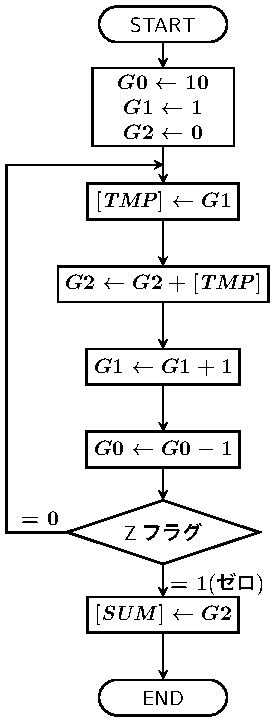
\includegraphics[scale=0.55]{../Tikz/flow3A.pdf}}
  \end{minipage}
  \begin{minipage}{0.36\columnwidth}
    {\ttfamily JZ使用(以前の例)\\\scriptsize
      \begin{tabular}{|l|l|l|}
              & LD     & G0, N    \\
              & LD     & G1, ONE  \\
              & LD     & G2, ZERO \\
              &        &          \\
      LOOP    & ST     & G1, TMP  \\
              & ADD    & G2, TMP  \\
              & ADD    & G1, ONE  \\
              & SUB    & G0, ONE  \\
              & JZ     & STOP     \\
              & JMP    & LOOP     \\
              &        &          \\
      STOP    & ST     & G2, SUM  \\
              & HALT   &          \\
              &        &          \\
      N       & DC     & 10       \\
      ONE     & DC     & 1        \\
      ZERO    & DC     & 0        \\
      TMP     & DS     & 1        \\
      SUM     & DS     & 1        \\
    \end{tabular}}
  \end{minipage}
  \begin{minipage}{0.36\columnwidth}
    {\ttfamily JNZ使用(改良版)\\\scriptsize
      \begin{tabular}{|l|l|l|}
              & LD     & G0, N    \\
              & LD     & G1, ONE  \\
              & LD     & G2, ZERO \\
              &        &          \\
      LOOP    & ST     & G1, TMP  \\
              & ADD    & G2, TMP  \\
              & ADD    & G1, ONE  \\
              & SUB    & G0, ONE  \\
              & JNZ    & LOOP     \\
              &        &          \\
              &        &          \\
              & ST     & G2, SUM  \\
              & HALT   &          \\
              &        &          \\
      N       & DC     & 10       \\
      ONE     & DC     & 1        \\
      ZERO    & DC     & 0        \\
      TMP     & DS     & 1        \\
      SUM     & DS     & 1        \\
    \end{tabular}}
  \end{minipage}
  \vfill
\end{frame}

%==============================================================================
\begin{frame}
  \frametitle{CMP(Compare)命令(比較命令)}
  レジスタの値とメモリの値を比較しフラグを変化させる.\\
  比較には引き算を使用する.
  \vfill
  \begin{description}
  \item[フラグ:] 計算結果により変化する.
    \vfill

  \item[ニーモニック:]\texttt{CMP GR,EA}~~~~~~~~~\texttt{(GR - [EA])}
    \vfill

  \item[命令フォーマット:] 2バイトの長さを持つ.\\
    \twoByte{$0101_2$}{\GR~\XR}{\A}
    \vfill

  \item[フローチャート:] 値を保存しない引き算の意味.\\
    \centerline{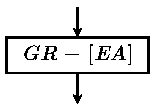
\includegraphics[scale=0.7]{../Tikz/cmp.pdf}}
  \end{description}
  \vfill
\end{frame}

%==============================================================================
\begin{frame}
  \frametitle{大小比較(演習問題の解答と同じ)}
  MとN大きい方を選択してLに格納する.\\
  \vfill
  \begin{minipage}{0.5\columnwidth}
    \centerline{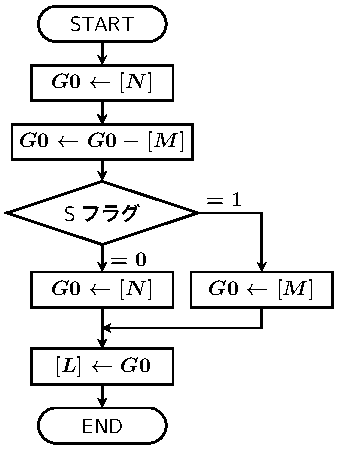
\includegraphics[scale=0.75]{../Tikz/flowI.pdf}}
  \end{minipage}
  \begin{minipage}{0.48\columnwidth}
    {\ttfamily\footnotesize
      \begin{tabular}{|l|l|l|}
              & LD     & G0, N    \\
              & SUB    & G0, M    \\
              & JM     & L1       \\
              &        &          \\
              & LD     & G0, N    \\
              & JMP    & L2       \\
              &        &          \\
      L1      & LD     & G0, M    \\
              &        &          \\
      L2      & ST     & G0, L    \\
              & HALT   &          \\
              &        &          \\
      N       & DS     & 1        \\
      M       & DS     & 1        \\
      L       & DS     & 1        \\
    \end{tabular}}
    \vfill
  \end{minipage}
\end{frame}

%==============================================================================
\begin{frame}
  \frametitle{大小比較(CMP,JNM 命令を使用して改良)}
  MとN大きい方を選択してLに格納する.\\
  \vfill
  \begin{minipage}{0.5\columnwidth}
    \centerline{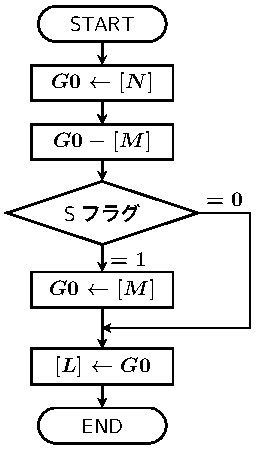
\includegraphics[scale=0.75]{../Tikz/flowJ.pdf}}
  \end{minipage}
  \begin{minipage}{0.48\columnwidth}
    {\ttfamily\footnotesize
      \begin{tabular}{|l|l|l|}
              & LD     & G0, N    \\
              & CMP    & G0, M    \\
              & JNM    & L1       \\
              &        &          \\
              & LD     & G0, M    \\
              &        &          \\
      L1      & ST     & G0, L    \\
              & HALT   &          \\
              &        &          \\
      N       & DS     & 1        \\
      M       & DS     & 1        \\
      L       & DS     & 1        \\
    \end{tabular}}
    \vfill
  \end{minipage}
\end{frame}

%==============================================================================
\begin{frame}
  \frametitle{まとめ}
  \emph{学んだこと}
  \begin{itemize}
  \item 今回の命令は,必須ではないが,あると便利なもの.
  \item 残りの条件ジャンプ命令(JNZ,JNC,JNM)
  \item 比較命令(CMP)
  \item 新しい命令を使用して改良したプログラム
  \end{itemize}
  \vfill

  \emph{演習(宿題)}
  \begin{itemize}
  \item \emph{割り算プログラム:}M番地のデータをN番地のデータで割り,
    商をK番地,余りをL番地に格納するプログラム
  \item データはどれも符号なし整数とする.
  \item 割り算は引き算の繰り返しでできる.
  \end{itemize}
  \vfill
\end{frame}

\end{document}
